\chapter{Experimental Vehicle}

In order to verify the approach we discuss in this theses, we needed a car-like robot which we could use for real-world testing. We took inspiration from the F1/10 competition \cite{F1/10}, the MIT RACECAR\footnote{https://mit-racecar.github.io/}, AutoRally\footnote{https://autorally.github.io/}, and other similar projects and we built a robot based on a chassis from an 1:10 scale \gls{RC} car with an on-board computer and a set of sensors. In this chapter, we will describe the hardware components we used to build our custom experimental vehicle.

\section{Chassis}

We used chassis, steering servo, \gls{DC} motor, \gls{ESC}, and a ratio transmitter and receiver from an off-the-shelf \gls*{RC} car. We removed the plastic cover and some unnecessary parts attached to the chassis and we attached a think plywood board on top of the chassis. We later mounted all of the electronics to the plywood board. Even though the weight of the battery and of the electronics is not negligible, the suspension of the vehicle is stiff enough to carry the weight without any significant roll and pitch changes during acceleration and cornering.

The chassis has the same geometry as a common passenger car with two fixed rear wheels and two front wheels with Ackermann steering geometry. All of the wheels are driven by the \gls*{DC} motor through a fixed gearbox. The wheels on both front and rear axes can move independently thanks to two differentials, one on each axis. The differentials are necessary for smooth travel during turns, when the outer wheel spins faster than the inner wheel.

The steering servo and the \gls*{ESC}, which controls the speed of the \gls*{DC} motor, both have a 3-pin connector which was originally connected to a radio receiver. Two of the pins connect to a \gls*{DC} power supply and the third connects to a signal wire. The signal is originally created by an radio transmitter which generates a \gls{PWM} signal. The \gls*{PWM} signal consists of pattern resembling a square wave, where the voltage measured on the signal wire is high (\SI{5}{\volt}) for some period of time and then the voltage drops to low (\SI{0}{\volt}) for the rest of the period. The pulse of high voltage lasts between \SI{1}{\milli\second} and \SI{2}{\milli\second} and the period of the signal is \SI{20}{\milli\second} as it is shown in Figure~\ref{fig:pwm}. We can therefore connect these connectors to a computer which generates appropriate signals to steer the vehicle. The \SI{20}{\milli\second} period of one \gls*{PWM} cycle gives us an upper limit of \SI{50}{\hertz} at which we can change the commands for the vehicle.


\begin{figure}[]\centering
	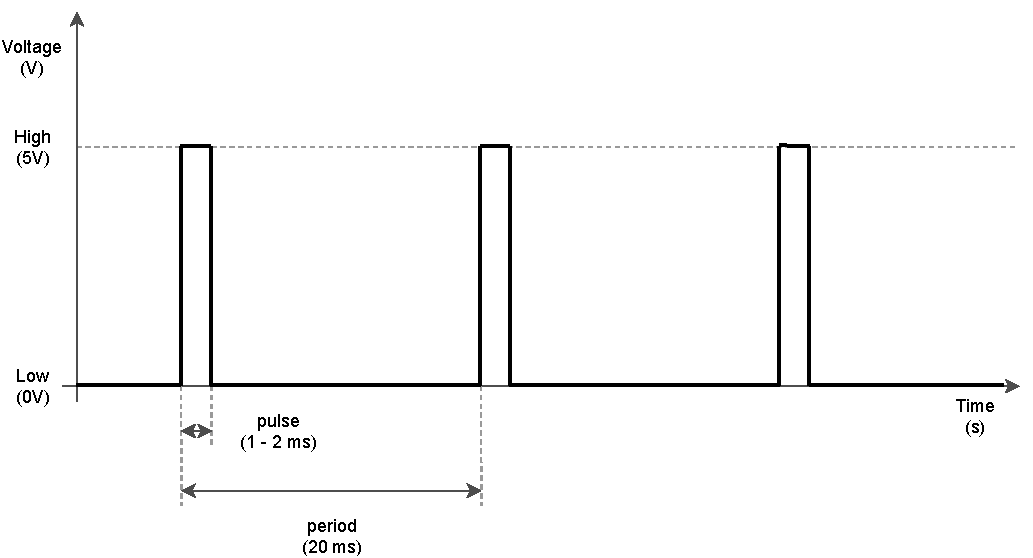
\includegraphics[width=125mm]{../img/pwm.pdf}
	\caption{The PWM signal for the steering servo and the ESC form a square wave with the period of \SI{20}{\milli\second} and pulse width between \SIlist{1;2}{\milli\second}.}
	\label{fig:pwm}
\end{figure}
\section{Sensors}

The vehicle uses on-board sensors to track its location on the racing track. We use a combination of three sensors: a \gls{LIDAR}, an \gls{IMU}, and a motor encoder. We tried several different sensors from different manufacturers, including \verb|Razor 9DoF IMU| and \verb|Scanse Sweep 2D LIDAR| but these devices did not yield good results. 

\paragraph{Hall Effect Encoder} consists of an 8-pole magnetic disc which we attach to the drive shaft of the vehicle, and a Hall effect sensor. The sensor sends a pulse every time it detects a change from a north pole to a south pole or vice-versa. This way we can detect that the motor has made one eigth of a revolution. By counting the number of revolutions and by assuming that the wheels of the vehicle roll perfectly against the road surface, we can estimate the distance that the vehicle traveled. By combining this information with the current steering angle of the front wheels, we can estimate the movement of the vehicle and use it as a source of odometry. We used a ``Wheel Encoder Kit from DAGU'' from SparkFun\footnote{https://www.sparkfun.com/products/12629}.

\paragraph{Bosch BNO055 USB Stick} is an \gls{IMU} which contains a triaxial accelerometer, a triaxial gyroscope, a triaxial magnetometer and a thermometer\footnote{https://www.bosch-sensortec.com/bst/products/all\_products/bno055} . We use the measurements of the gyroscope and the accelerometer to determine the acceleration of the vehicle to improve our odometry from the motor encoder, which cannot detect wheel skidding.

\paragraph{YDLIDAR X4} is a low-cost \ang{360} \gls{LIDAR} laser scanner. We use it to determine the distance to the surrounding obstacles. This sensor has a range of up to \SI{10}{\meter} and it takes \num{5000} samples every second while spinning at the frequency of almost \SI{12}{\hertz}. This sensor is connected to a computer via a micro-USB port and it is connected to a \SI{5}{\volt} power supply through a second micro-USB port.

\section{On-board Computer}

The brains of our autonomous vehicle is the NVIDIA Jetson Nano\footnote{https://developer.nvidia.com/embedded/jetson-nano-developer-kit} . This board contains a quad-core ARM A57 with the clock frequency of \SI{1.43}{\giga\hertz}, \SI{4}{\giga B} of LPDDR4 RAM and a 128-core Maxwell GPU. This computer is powered through a Micro-USB port with \SI{5}{\volt}/\SI{2}{\ampere}\footnote{The board can operate with a lower power consumption of \SI{5}{\watt} in a mode in which two of the CPU cores are turned off.}. The Jetson has 4 USB ports which are used to connect the \gls*{LIDAR}, the \gls*{IMU}, and two Arduino boards. The board does not include a Wi-Fi antena and therefore we added an Intel Dual Band Wireless-Ac 8265 W/Bt card to the M.2 slot of the board in order to receive telemetry while the vehicle is driving along a circuit.

\subsection{Microcontrollers}

We use two Arduino Nano boards\footnote{https://www.arduino.cc/en/Guide/ArduinoNano} as an interface between the actuators, the radio receiver, and the motor encoder, and the Jetson Nano board.

\paragraph{Hall Effect Encoder} is connected to an interrupt pin of one Arduino and this Arduino counts the number of revolutions of the motor. This board also provides power to the Hall sensor.

\paragraph{ESC and Servo} are connected to \gls{PWM} output pins of the other Arduino board and the radio receiver is connected to two interrupt pins. This board contains logic which converts high-level commands for the actuators into corresponding \gls*{PWM} signals. It also contains a safety mechanism which disables autonomous mode of the vehicle and allows the supervisor to take over control of the vehicle when he or she uses the remote controller.

\section{Power Supply}

The \gls*{DC} motor and the servo are powered by \SI{7.2}{\volt} \SI{5000}{\milli\ampere\hour} NiMH battery which was included with the \gls*{RC} car. The rest of the electronics of the vehicle is powered by a regular \SI{20000}{\milli\ampere\hour} power bank which has two output USB ports. One of these ports can supply \SI{2}{\ampere} and the Jetson Nano board is connected to it, the other port can supply \SI{1}{\ampere} and it powers the \gls*{LIDAR}.

This setup ensures that the power in the batteries supplying the motors of the vehicle discharge much sooner than the power bank which supplies the computer and sensors if we start with fully charged batteries. It should never occur that the computer shuts down while the car is being driven autonomously and it will not continue moving uncontrollably. We also do not need to build a custom power delivery board.